\chapter{Design and implementation}\label{DesignAndImplementation}
\ifpdf
    \graphicspath{{Chapter3/Chapter3Figs/PNG/}{Chapter3/Chapter3Figs/PDF/}{Chapter3/Chapter3Figs/}}
\else
    \graphicspath{{Chapter3/Chapter3Figs/EPS/}{Chapter3/Chapter3Figs/}}
\fi

The aim of this chapter is to give a thorough description of our concrete implementation of the theoretical framework introduced
in Chapter \ref{TheoreticalFramework}. We list and provide an explanation of the individual
components and also explain our reasoning for certain design choices. In section \ref{WebApp} we present a proof-of-concept web application that 
we have developed in order to demonstrate how the different components can be integrated together to form a platform for event detection. 

\section{System Overview}
Figure \ref{SystemOverview} shows an overview of the system architecture which is a pipeline of the individual components we described
in Chapter \ref{TheoreticalFramework}. Each one of these components is depicted as an independent module in the figure.  
Initially, historical tweets from a service provider (Twitter API or another provider) are retrieved and stored in an 
appropriate format in the database. Subsequently, the system receives a stream of tweets from the database and processess and 
transforms them in a format that is appropriate for clustering. The next step in the pipeline is the actual clustering of the tweets 
in order to detect groups of tweets discussing the same topic. Then, the extracted clusters are processed in order to identify the events 
and generate their summaries. Finally, a visual representation of the results should be generated in order to aid understanding of the events.\\

\begin{figure}[!htbp]
  \begin{center}
    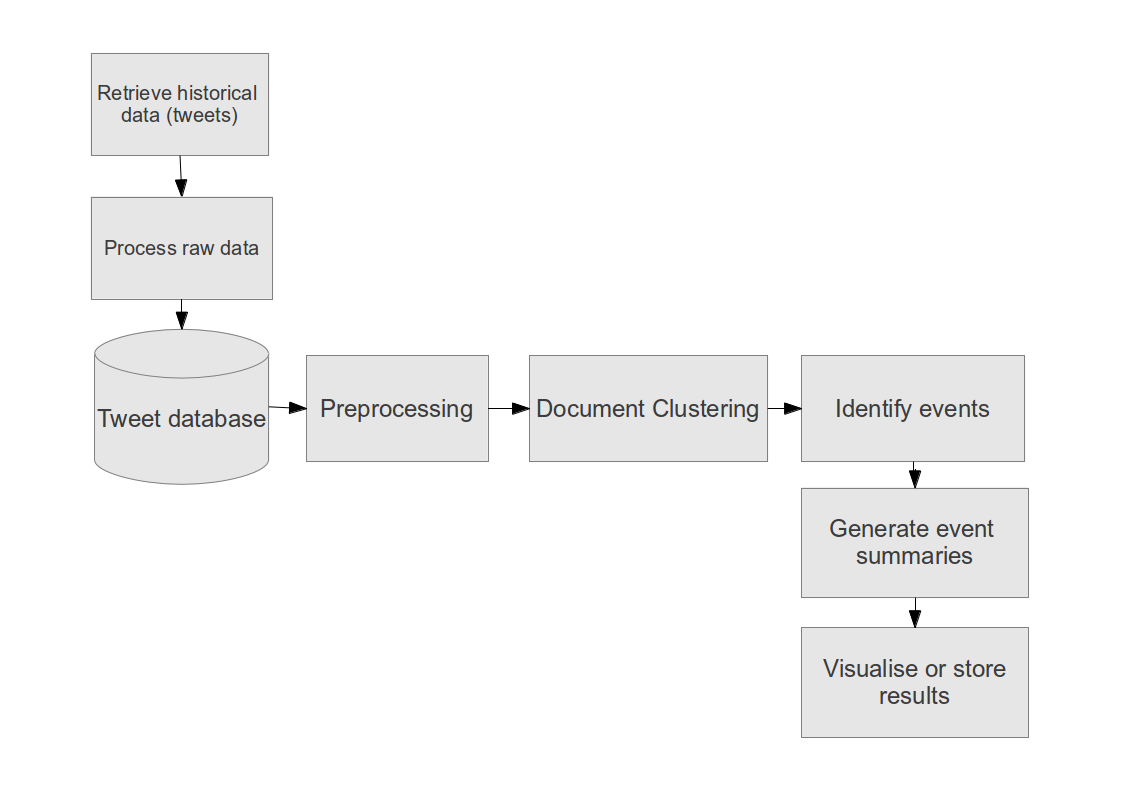
\includegraphics[height=3in, width=6in]{system-overview}
    \caption{System overview - The event extraction system comprises of several independent components.}
    \label{SystemOverview}
  \end{center}
\end{figure}

\section{Tools}
In the process of implementing the system we have mainly used our implementation of the algorithms but several third-party 
software libraries were used to implement sub-components of the system. Here we describe the main tools we have used.\\ 


\section{Data Retrieval and Preprocessing}


\section{Clustering}

\section{Identifying events}

\section{Generating automatic summaries}

\section{Classifying users}

\section{Optimisations}

\section{Developing a proof-of-concept web application}\label{WebApp}

\section{Summary}

% ------------------------------------------------------------------------


%%% Local Variables: 
%%% mode: latex
%%% TeX-master: "../thesis"
%%% End: 
